Noria without partial state, as described in \S\ref{s:noria}, uses significant
amounts of memory. All results for all queries must be materialized, and unlike
traditional caching approaches, unimportant cached results are not evicted to
free up memory. To address the high memory use of traditional materialized
views, this thesis proposes \textit{partially materialized state}. Partial state
enables Noria to store and maintain only a subset of a materialized view's
contents, and to compute missing state on demand. Partial state also enables
Noria to implement eviction, so that the materialization cost is kept low even
as the underlying workload changes.

This chapter discusses the partially stateful model and its components. The next
chapter examines the practical challenges that arise when partial state is
implemented in a dataflow system.

\section{Missing State}

Partial state allows state to be \textit{missing}. Missing state indicates that
a particular value is not yet known, and must be computed on demand if the
application queries for it. State can be marked as missing both in state that is
internal to the dataflow, like the state of an aggregation, and in externally
visible state like Noria's query result caches.

With partial state, most Noria state starts out as missing, and is populated
driven by what data the application queries for. This also allows Noria to
quickly adopt new views, since in the common case no computation need happen
when additional operators are added.

\begin{figure}
  \centering
  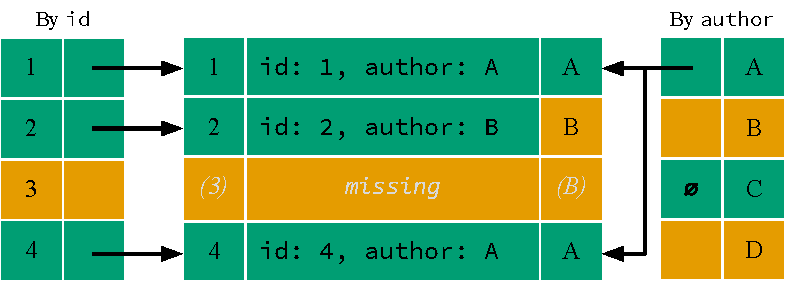
\includegraphics{diagrams/Indexing.pdf}
  \caption{Multiple indexes over the state in a single view in Noria. Even
  though \emph{some} rows for author B are present, some are missing and so the
  entry for B is considered missing in the \texttt{author} index. Even though no
  rows for author C are present, the index entry is not marked as missing, which
  would happen if Noria has checked that there are indeed no rows for
  author C.}
  \label{f:indexing}
\end{figure}

Missing state manifests as missing entries in particular indices. Indexes over a
given state are either all partial or none of them are. This may seem strange
based on how indices work in traditional relation databases.
Figure~\vref{f:indexing} gives an example with two different partial indices
over a view that holds a unique story identifier and the story's author. One
index is over the primary key column \texttt{id}, and one is over the story
author. Here, even though some rows with author B are present, the index entry
for author B is still considered missing, since not \emph{all} rows with author
B are present. This is necessary, as otherwise an application query for stories
authored by B would return an incomplete, and hence incorrect, result.
Similarly, while there are no rows for authors C or D, C is considered complete
because Noria has checked upstream that there are indeed no stories written by
C.

If, while processing an update, Noria encounters missing state, this indicates
that the update does not affect query results that the application has indicated
interest in. In such a case, Noria has two options: eagerly compute the missing
state before proceeding, or discard the update. To avoid unnecessarily
maintaining unimportant cached results, Noria drops updates in this case.

An important corollary of the above is that partial state must be enabled
on all stored state \emph{below} any partial state. It is illegal for the
dataflow to contain state for two nodes $A$ and $B$ where $A$ is an ancestor of
$B$, $A$ uses partial state, and $B$ does not use partial state. To see why,
consider what would happen if an update arrives at $A$ for a missing entry. $A$
would discard that update, and $B$'s state would remain perpetually stale.

\section{Upqueries}
\label{s:upqueries}

If an application requests data that is found to be missing, Noria issues an
\textit{upquery} to compute the requested data. Upqueries flow ``up'' the
dataflow graph, towards the base tables at the ``top'', and constitute a request
for the target of the upquery to replay past data. Upqueries may recurse if the
requested state is not available at the initial target.

The response to an upquery takes the form of a regular dataflow update that
flows down the dataflow. It combines all past deltas pertinent to the upquery
into a single update, and holds only positive deltas that represent the current
set of relevant records.

Operators are generally not aware whether they are processing an update that
resulted from a base table change or an upquery. The upquery response flows
in-line with other dataflow updates, and follows the edges of the dataflow.

Upquery responses are special in two key ways. First, they only propagate along
edges towards the operator that issued the upquery, so that one upquery does not
populate the relevant data in the state of \emph{every} operator. And second,
if an operator encounters missing state while processing an upquery response
update, it does not discard that update, but instead does the work necessary to
process that update. This process is described in further detail below.

When an application query encounters missing state in a view, Noria needs to
know what upqueries to issue. The set of necessary upqueries for each view is
that view's \textit{upquery plan}. Noria determines upquery plans by analyzing
each view's query when the application first installs that view, and deciding
how best to recompute its results. It does so by finding all \emph{possible}
upquery plans, choosing among them, and then informing all involved domains of
the chosen plan. There may be multiple possible candidates if there are multiple
equivalent ways to compute the missing state, such as by changing the direction
in which joins are executed as explained below.

\subsection{Key Provenance Tracing}

To determine what upqueries can be issued to reconstitute missing entries in a
given index, Noria must trace the view's parameter column back to a column in
upstream state. The intuition here is that in order to answer the application's
query of ``give me the results where column $C$ has value $x$'', Noria must be
able to replay rows where $C = x$ from somewhere. Or, phrased differently, when
the output for $C = x$ is missing, Noria must have a way to get at the inputs
that \emph{generate} $C = x$. As an example, if a view counts books by a given
author, and the current count for author $a$ is missing, Noria must be able to
somehow produce all books by author $a$.

\begin{figure}[t]
  \centering
  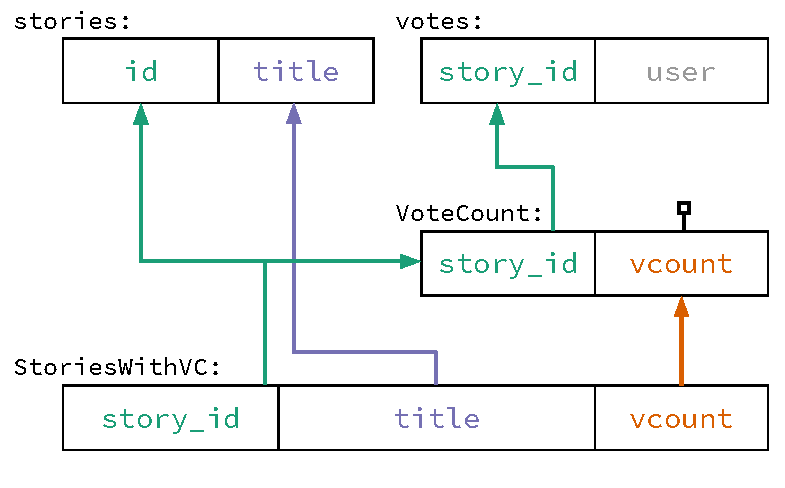
\includegraphics{diagrams/Key Provenance.pdf}
  \caption{Key provenance for each column in the \texttt{StoriesWithVC} view
  from Listing~\ref{l:vote-src}. Notice that \texttt{story\_id} has multiple
  base table origins, and \texttt{vcount} does not trace back to any base table
  columns. The query only uses \texttt{story\_id} as a parameter, so only its
  provenance is used to choose the upquery path.}
  \label{f:key-prov}
\end{figure}

More generally, in order to recompute the results where $C = x$ in some view
$V$, Noria must determine the \textit{key provenance} of $C$; where $C$ ``came
from''. Noria computes key provenance by tracing columns ``up'' the dataflow to
where they originate, which results in a provenance graph like the one shown in
Figure~\vref{f:key-prov} for the \texttt{StoriesWithVC} view from
Listing~\vref{l:vote-src}. The figure illustrates two important properties of
key tracing:

\begin{enumerate}
  \item An output column may trace to multiple input columns if it corresponds
    to the join column in a join, or if it passes through a union. The
    provenance of the \texttt{story\_id} column, for example, traces both to
    \texttt{stories.id} and \texttt{votes.story\_id}.
  \item An output column may be entirely computed, and thus have no association
    with a column in the inputs. The \texttt{vcount} column is computed by the
    \texttt{VoteCount} aggregation, and does not exist in the input data set.
\end{enumerate}

In Listing~\ref{l:vote-src}, Noria is asked to parameterize
\texttt{StoriesWithVC} by the \texttt{story\_id} column. The key provenance
graph tells Noria that it can request input data for a given \texttt{story\_id}
by sending an upquery either to the \texttt{stories} table using the \texttt{id}
column, or to the \texttt{vote} table using the \texttt{story\_id} column. Since
there exists a way to replay the input data for a missing output entry in this
case, the \texttt{StoriesWithVC} view can be made partial.

\paragraph{Broken Provenance.}
Consider what would happen if Listing~\ref{l:vote-src} had \texttt{WHERE vcount
= ?} as its parameter instead. If an application query misses in that case, the
upquery would have to be sent to \texttt{VoteCount}, and query for ``all stories
whose vote count is $x$''. If that state is present, all is well, but if
\texttt{VoteCount} is missing the state for \texttt{vcount = x}, there's a
problem. Noria now has no way to compute the missing state except by replaying
\emph{all} state in \texttt{vote} without an index. This would be equivalent to
a full table scan in a traditional database.
Noria's only%
%
\footnote{Noria cannot disable partial state just for \texttt{StoriesWithVC},
since that would violate place a partial index above a non-partial index, which
is illegal.}
%
efficient option is to disable partial
state for \texttt{VoteCount}. This ensures that any upquery to it never misses,
and therefore a table scan is never needed. Instead, the table scan is performed
only once: when the view is initially added. But this comes at the cost of
maintaining the entire resultset of the query for all parameter values.

\paragraph{Asymmetric Provenance.}
The join in Listing~\ref{l:vote-src} uses a inner join ($\bowtie$), and Noria is
therefore free to upquery \emph{either} side. If it upqueries the ``left'' side
of the join, the regular processing pipeline will perform the necessary lookups
into the ``right'' side of the join, and vice-versa. However, if the view query
used a left or right \emph{outer} join, Noria must upquery a particular side of
the join. For a left join, it must upquery the left ancestor, or risk missing
rows in the left ancestor that have no matching rows in the right ancestor. For
a right join, the same logic applies, but mirrored to the right ancestor.

\paragraph{Disjoint Provenance.}
If the provenance of a column crosses a union, \emph{all} ancestors of that
union must be upqueried, as opposed to just one as is the case with upqueries
through a join. Unlike with a join, the regular dataflow processing of the
upquery response through a union will not bring along results from the other
ancestors, so the requesting operator must ask them all individually.

\subsection{Path Selection}
\label{s:upquery:selection}

Once Noria has obtained a set of candidate upquery paths through key provenance,
it must decide on an upquery plan based on those paths. If there is only one
candidate, the choice is trivial. But with symmetric joins, multiple candidate
paths may be generated. Here, Noria is free to use whatever heuristics it sees
fit to decide which side of a symmetric join to send upqueries to. For example,
it may choose to send upqueries to the larger of the joined inputs so that fewer
lookups are necessary when processing the response.

In addition, key provenance tracing produces upquery paths that reach all the
way back to the origin of a column, which is usually located at the base tables.
However, it would be inefficient for operators to issue upqueries all the way to
the base tables on every miss. Some intermediate state may already have the
necessary data, and the upquery data could be sourced from there instead. Noria
therefore trims the paths from key provenance such that only the suffix of
operators starting at the last materialized state are included. For example, in
Figure~\ref{f:key-prov}, if Noria decides to upquery \texttt{StoriesWithVC}
through \texttt{VoteCount}, the upquery path would source its data from
\texttt{VoteCount}, not from \texttt{votes}.

If an upquery reaches its origin and finds that the requested state is missing
there too, a second upquery is issued using the origin's upquery paths, and only
when that upquery resolves does the original upquery resume. Upqueries may
recurse all the way up to the base tables this way, but avoid doing so if any
intermediate state can be re-used.

This process leaves Noria with a set of paths to upquery when it encounters a
missing entry in a given state.

\subsection{Implementing a Plan}

Once Noria has decided on a plan, that plan is communicated to all domains
that appear along each path in the plan. This is necessary so that each domain
knows where to route upquery responses that are part of a given plan, and does
not disseminate the response to the entire downstream dataflow.

When Noria announces the upquery plan, it may also add additional indices
to existing state to facilitate efficient execution of the new upqueries. In
particular, when an upquery arrives at the materialization it wants to source
data from, Noria needs an efficient way to find the requested data. Concretely,
Noria needs an index on the materialization whose key matches the lookup key of
the upquery. In this way, upquery plans adds additional indexing obligations
that Noria must take into account.

The key provenance information from Figure~\vref{f:key-prov} gives Noria all the
information it needs to set up these indexes: an index is needed on the upquery
key column on each state on the chosen upquery paths. In the case of the view
from Listing~\ref{l:vote-src}, an index is needed on
\texttt{StoriesWithVC.story\_id}, as well as either \texttt{stories.id} or both
\texttt{VoteCount.story\_id} and \texttt{votes.story\_id}\footnote{An index is
needed on \texttt{votes.story\_id} since the upquery to \texttt{VoteCount} may
recurse.}, depending on which upquery path Noria chooses across the join.

\section{Eviction}

Over time, the subset of data that the application cares about tends to change.
When it does, query results that were accessed previously may no longer be
important to maintain as they are no longer accessed. Partial state allows Noria
to cater to such changing application patterns by \textit{evicting} state
entries after they have been computed. When an entry is evicted, it is marked as
missing, and subsequent requests for that state trigger an upquery as usual for
missing state.

When Noria evicts an entry from state in the middle of the dataflow, the missing
entry may cause an update to be discarded even though downstream entries hold
data that would grow stale without that update. For example, consider what
happens if an operator counts the number of votes per author, and contains a
count of 7 for the author ``Jane''. Then, the state for ``Jane'' is evicted from
some operator upstream of the count. If an update now arrives at the operator
where ``Jane'' is missing; it would discard the update, and the downstream count
would remain perpetually stale.

To avoid such permanently stale entries, Noria must ensure that when an entry is
evicted, any dependent state downstream is also evicted. More formally, it must
ensure that:

\begin{invariant}
  \label{i:missing-suffix}
  If an operator encounters a missing state entry while processing a record $r$
  in an update, any downstream state that reflects $r$ must be evicted.
\end{invariant}

Upqueries as described thus far, without evictions, generally uphold this
invariant\footnote{Though not always; see \S\ref{join-evictions}}. As upqueries
recurse up the dataflow, missing state is filled in ``from the top down'' until
the operator that originally issued the upquery is presented with the requested
state. Any misses that occur during the processing of an upquery causes
recursive upqueries, which fill that missing state before proceeding.

To uphold the property in the face of evictions, Noria issues evictions
downstream whenever it decides to evict entries from state in the middle of the
graph. This ensures that any future update that touches the evicted state can
safely be discarded, as any relevant downstream state has been discarded as
well.

Invariant~\ref{i:missing-suffix} implies the corollary from earlier that partial
state cannot exist upstream of non-partial state. Since state cannot be evicted
from non-partial state, Noria would be unable to satisfy the invariant should it
ever encounter missing state upstream of the non-partial state.
